\documentclass[12pt,a4paper]{article}
\usepackage{rmpackages}																% usual packages
\usepackage{rmtemplate}																% graphic charter
\usepackage{rmexocptce}																% for DS with cptce eval

%\cfoot{} 													% if no page number is needed
\renewcommand\arraystretch{1.25}		% stretch table line height

\begin{document}

\begin{header}
Interrogation -- Chapitre 4

\normalsize
\flushleft
\begin{doublespace}
Classe :

NOM :

\end{doublespace}
Prénom : 
\end{header}

\section*{Données}

\begin{center}
\begin{tabular}{ll}
Masse du proton 		& $m_\mathrm{p} = \unit{1{,}673 \times 10^{-27}}{kg}$ \\
Masse du neutron	& $m_\mathrm{n} = \unit{1{,}675 \times 10^{-27}}{kg}$ \\
Masse de l'électron	& $m_\mathrm{e} = \unit{9{,}1 \times 10^{-31}}{kg}$ \\
Rayon de l'atome de béryllium & $r_\mathrm{atome} = \unit{110}{pm} $ \\
Rayon d'un noyau de béryllium & $r_\mathrm{noyau} = \unit{2{,}5\times 10^{-15}}{m} $
\end{tabular}

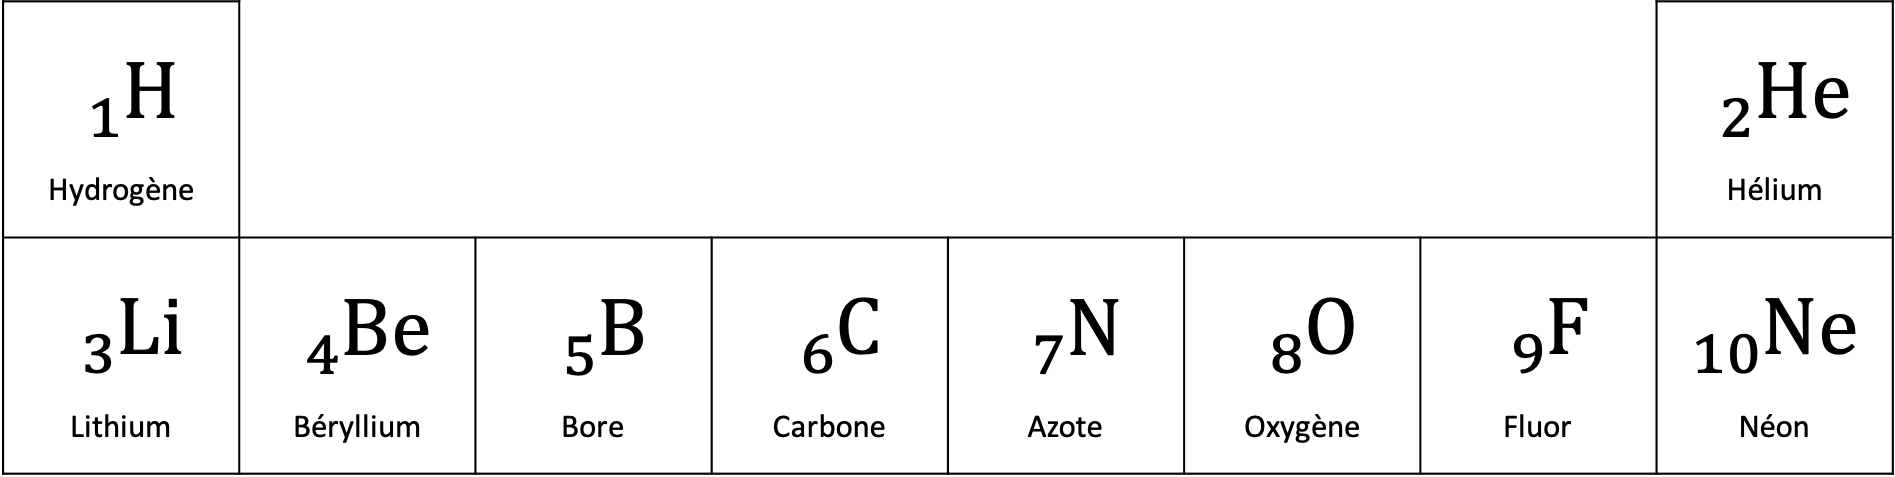
\includegraphics[scale=0.5]{images/periodic_table_2.png}
\end{center}

\begin{exo}{Identifier un atome}

\begin{multicols}{2}
\begin{center}
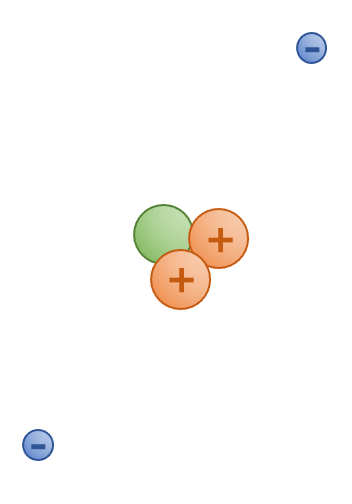
\includegraphics[scale=1]{images/he3.png}
\end{center}

\begin{enumerate}
\item \rco{} \ajrco{1}

Légender le modèle ci-contre.

\item \com{} \ajcom{1}

Justifier qu'il s'agit du modèle d'un atome.

\item \rea{} \ajrea{1}

Donner l'écriture conventionnelle de son noyau.

\item \rea{} \ajrea{1}

Calculer la masse de cet atome en utilisant les valeurs les plus précises possibles.
\end{enumerate}
\end{multicols}
\end{exo}

\begin{exo}{Écriture conventionnelle}


\begin{enumerate}
\item \app{} \ajapp{2}

Compléter le tableau ci-dessous.
\end{enumerate}

\begin{center}
\renewcommand\arraystretch{2}		% stretch table line height
\begin{tabular}{|l|c|c|c|c|}
\hline
\textbf{Symbole de l'élément}	& \quad{} B \quad{} & \quad{} F \quad{} & \quad{} H \quad{} & \quad{} Cr \quad{} \\
\hline
\textbf{Nombre de protons}		& 4 & 9 & ... & 24 \\
\hline
\textbf{Nombre de neutrons}	& ... & 10 & 2 & ... \\
\hline
\textbf{Écriture conventionnelle du noyau} & $^{9}_{...}\text{B}$ & ... & $^{...}_{1}\text{H}$ & $^{52}_{...}\text{Cr}$ \\
\hline
\end{tabular}
\renewcommand\arraystretch{1.5}		% stretch table line height
\end{center}

Comme indiqué dans le tableau, l'atome de fluor (F) possède 9 protons et 10 neutrons.
Il peut gagner un électron pour former l'ion fluorure.

\begin{enumerate}[resume]
\item \anarai{} \ajanarai{1}

Donner en la justifiant la composition de l'ion fluorure.

\item \anarai{} \ajanarai{0.5}

L'ion fluorure est-il un anion ou un cation ?

\item \rea{} \ajrea{0.5}

Donner la formule chimique de l'ion fluorure.
\end{enumerate}
\end{exo}

\begin{exo}{Comparaison}
\begin{enumerate}
\item \rea{} \ajrea{1.5}

Comparer le rayon de l'atome de béryllium et celui de son noyau.

\emph{Rappel : $\unit{1}{pm} = \unit{1\times 10^{-12}}{m}$.}

\item \val{} \ajval{0.5}

Ce résultat est-il surprenant ?
Justifier.
\end{enumerate}

\end{exo}

\vfill
\makecptces

\end{document}